\section{Handkenmerken en controle in de tool}\label{app:feature-tool}
De tool vergelijkt gemeten kenmerken met het werkboek voor een gekozen letter. Deze doelletter beïnvloedt de controle, niet de voorspelling van het getrainde model. Een overeenkomst betekent dat de meting aan de ingestelde regel voldoet; zij valideert geen anatomie of correcte ASL-uitvoering.

Een interne gewrichtshoek wordt berekend tussen de twee segmenten rond het middelste handpunt; een rechte vinger nadert $180^\circ$. MCP is de knokkel, PIP het middelste gewricht en DIP het eindgewricht; de duim heeft een IP. De metingen gebruiken geschatte wereldhandpunten. MCP-hoeken en duimvorm zijn geometrische benaderingen, geen klinische metingen.

\begin{table}[h]\centering\small
\caption{Belangrijkste regels in \texttt{config/thresholds.json} voor de werkboekcontrole. Dit zijn projectkeuzes, geen universele normen.}
\begin{tabular}{p{.19\linewidth}p{.72\linewidth}}\toprule
Kenmerk & Meetregel\\\midrule
Vingerbuiging & Gebogen bij hoogstens $130^\circ$, gestrekt vanaf $150^\circ$; daartussen deels gebogen. De duim-IP gebruikt $80^\circ$ en $155^\circ$.\\
Spreiding & Genormaliseerde ruimte minstens 0,25, diepteverschil hoogstens 0,6, richtingscosinus positief en PIP/DIP-hoeken minstens $120^\circ$. Uitwaaieren is toegestaan.\\
Vermoede kruising & Laterale omwisseling langs het vingerprofiel, diepteverschil hoogstens 0,7 en voldoende strekking. Alleen kruisende 2D-lijnen zijn onvoldoende.\\
Duimvorm & B-vormig bij een getekende palmgerichte duimafwijking groter dan $16^\circ$; anders niet B-vormig.\\
Contact & Vingertopafstand gedeeld door pols--middelvingerbasis. Contact bij ratio hoogstens 0,1; nabij tot en met 0,825; daarboven veraf.\\\bottomrule
\end{tabular}\end{table}

Het werkboek kan meerdere toegestane categorieën bevatten. Bij ``geen contact'' zijn nabij en veraf beide geldig. Onbekende metingen worden niet als bevestigde overeenkomst beoordeeld; lege referentievelden tellen niet mee. De tool maakt zo zichtbaar welke regels wel en niet overeenkomen, los van de uiteindelijke lettervoorspelling.

\begin{figure}[h]\centering
\IfFileExists{figures/feature_tool_screenshot.png}{%
  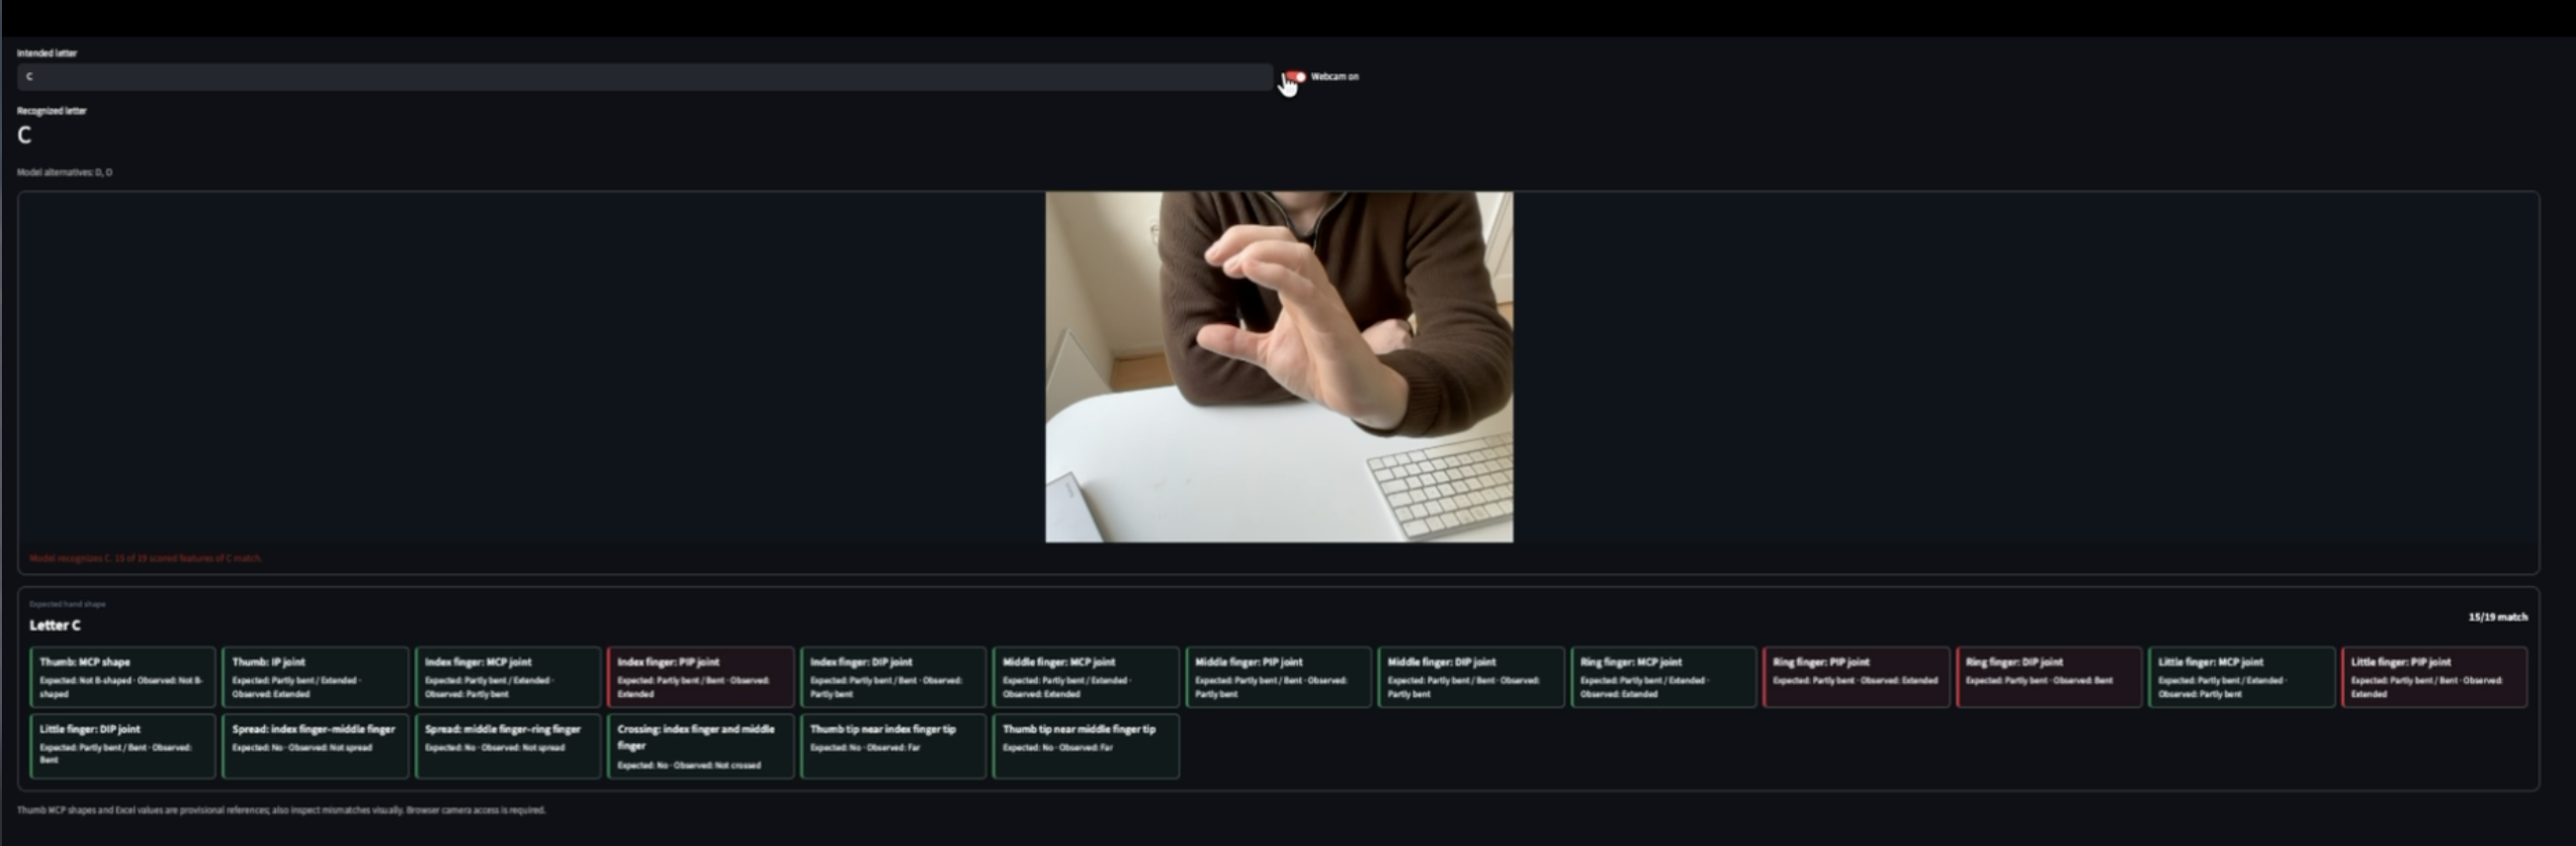
\includegraphics[width=.95\linewidth,height=.5\textheight,keepaspectratio]{figures/feature_tool_screenshot.png}%
}{%
  \fbox{\begin{minipage}[c][4.5cm][c]{.90\linewidth}\centering
  \textbf{TODO: eigen foto of screenshot van de featuretool}\\[1em]
  Toon de handpunten, gekozen letter en verwachte/gemeten kenmerken.\\[1em]
  Bestand: \texttt{figures/feature\_tool\_screenshot.png}
  \end{minipage}}%
}
\caption{Invoegplek voor de featuretool. \textbf{TODO:} voeg de eigen opname toe en pas het bijschrift aan de zichtbare letter en uitkomst aan. Groen betekent overeenkomst met het werkboek, rood een afwijking.}
\label{fig:feature-tool-screenshot}
\end{figure}

De functies \texttt{measure\_hand\_features}, \texttt{categorize\_workbook\_features} en \texttt{live\_feature\_rows} berekenen en vergelijken de kenmerken. De tool kan met \texttt{--capture} een opgeslagen opname openen zonder camera of training. Het plaatsen van het genoemde afbeeldingsbestand vervangt de placeholder bij compileren automatisch.
